%!TeX root=../sensetop.tex
\chapter[Chapter \thechapter]{}
\lettrine[lraise=0.3]{M}{rs} John Dashwood now installed herself mistress of Norland; and her mother and sisters-in-law were degraded to the condition of visitors. As such, however, they were treated by her with quiet civility; and by her husband with as much kindness as he could feel towards anybody beyond himself, his wife, and their child. He really pressed them, with some earnestness, to consider Norland as their home; and, as no plan appeared so eligible to Mrs Dashwood as remaining there till she could accommodate herself with a house in the neighbourhood, his invitation was accepted.

A continuance in a place where everything reminded her of former delight, was exactly what suited her mind. In seasons of cheerfulness, no temper could be more cheerful than hers, or possess, in a greater degree, that sanguine expectation of happiness which is happiness itself. But in sorrow she must be equally carried away by her fancy, and as far beyond consolation as in pleasure she was beyond alloy.

Mrs John Dashwood did not at all approve of what her husband intended to do for his sisters. To take three thousand pounds from the fortune of their dear little boy would be impoverishing him to the most dreadful degree. She begged him to think again on the subject. How could he answer it to himself to rob his child, and his only child too, of so large a sum? And what possible claim could the Miss Dashwoods, who were related to him only by half blood, which she considered as no relationship at all, have on his generosity to so large an amount. It was very well known that no affection was ever supposed to exist between the children of any man by different marriages; and why was he to ruin himself, and their poor little Harry, by giving away all his money to his half sisters?

<It was my father's last request to me,> replied her husband, <that I should assist his widow and daughters.>

<He did not know what he was talking of, I dare say; ten to one but he was light-headed at the time. Had he been in his right senses, he could not have thought of such a thing as begging you to give away half your fortune from your own child.>

<He did not stipulate for any particular sum, my dear Fanny; he only requested me, in general terms, to assist them, and make their situation more comfortable than it was in his power to do. Perhaps it would have been as well if he had left it wholly to myself. He could hardly suppose I should neglect them. But as he required the promise, I could not do less than give it; at least I thought so at the time. The promise, therefore, was given, and must be performed. Something must be done for them whenever they leave Norland and settle in a new home.>

<Well, then, \textit{let} something be done for them; but \textit{that} something need not be three thousand pounds. Consider,> she added, <that when the money is once parted with, it never can return. Your sisters will marry, and it will be gone for ever. If, indeed, it could be restored to our poor little boy\longdash>

<Why, to be sure,> said her husband, very gravely, <that would make great difference. The time may come when Harry will regret that so large a sum was parted with. If he should have a numerous family, for instance, it would be a very convenient addition.>

<To be sure it would.>

<Perhaps, then, it would be better for all parties, if the sum were diminished one half.—Five hundred pounds would be a prodigious increase to their fortunes!>

<Oh! beyond anything great! What brother on earth would do half so much for his sisters, even if \textit{really} his sisters! And as it is—only half blood!—But you have such a generous spirit!>

<I would not wish to do any thing mean,> he replied. <One had rather, on such occasions, do too much than too little. No one, at least, can think I have not done enough for them: even themselves, they can hardly expect more.>

<There is no knowing what \textit{they} may expect,> said the lady, <but we are not to think of their expectations: the question is, what you can afford to do.>

<Certainly—and I think I may afford to give them five hundred pounds a-piece. As it is, without any addition of mine, they will each have about three thousand pounds on their mother's death—a very comfortable fortune for any young woman.>

<To be sure it is; and, indeed, it strikes me that they can want no addition at all. They will have ten thousand pounds divided amongst them. If they marry, they will be sure of doing well, and if they do not, they may all live very comfortably together on the interest of ten thousand pounds.>

<That is very true, and, therefore, I do not know whether, upon the whole, it would not be more advisable to do something for their mother while she lives, rather than for them—something of the annuity kind I mean.—My sisters would feel the good effects of it as well as herself. A hundred a year would make them all perfectly comfortable.>

His wife hesitated a little, however, in giving her consent to this plan.

<To be sure,> said she, <it is better than parting with fifteen hundred pounds at once. But, then, if Mrs Dashwood should live fifteen years we shall be completely taken in.>

<Fifteen years! my dear Fanny; her life cannot be worth half that purchase.>

<Certainly not; but if you observe, people always live for ever when there is an annuity to be paid them; and she is very stout and healthy, and hardly forty. An annuity is a very serious business; it comes over and over every year, and there is no getting rid of it. You are not aware of what you are doing. I have known a great deal of the trouble of annuities; for my mother was clogged with the payment of three to old superannuated servants by my father's will, and it is amazing how disagreeable she found it. Twice every year these annuities were to be paid; and then there was the trouble of getting it to them; and then one of them was said to have died, and afterwards it turned out to be no such thing. My mother was quite sick of it. Her income was not her own, she said, with such perpetual claims on it; and it was the more unkind in my father, because, otherwise, the money would have been entirely at my mother's disposal, without any restriction whatever. It has given me such an abhorrence of annuities, that I am sure I would not pin myself down to the payment of one for all the world.>

<It is certainly an unpleasant thing,> replied Mr Dashwood, <to have those kind of yearly drains on one's income. One's fortune, as your mother justly says, is \textit{not} one's own. To be tied down to the regular payment of such a sum, on every rent day, is by no means desirable: it takes away one's independence.>

<Undoubtedly; and after all you have no thanks for it. They think themselves secure, you do no more than what is expected, and it raises no gratitude at all. If I were you, whatever I did should be done at my own discretion entirely. I would not bind myself to allow them any thing yearly. It may be very inconvenient some years to spare a hundred, or even fifty pounds from our own expenses.>

<I believe you are right, my love; it will be better that there should be no annuity in the case; whatever I may give them occasionally will be of far greater assistance than a yearly allowance, because they would only enlarge their style of living if they felt sure of a larger income, and would not be sixpence the richer for it at the end of the year. It will certainly be much the best way. A present of fifty pounds, now and then, will prevent their ever being distressed for money, and will, I think, be amply discharging my promise to my father.>

% \begin{figure}[t]
% \centering
% 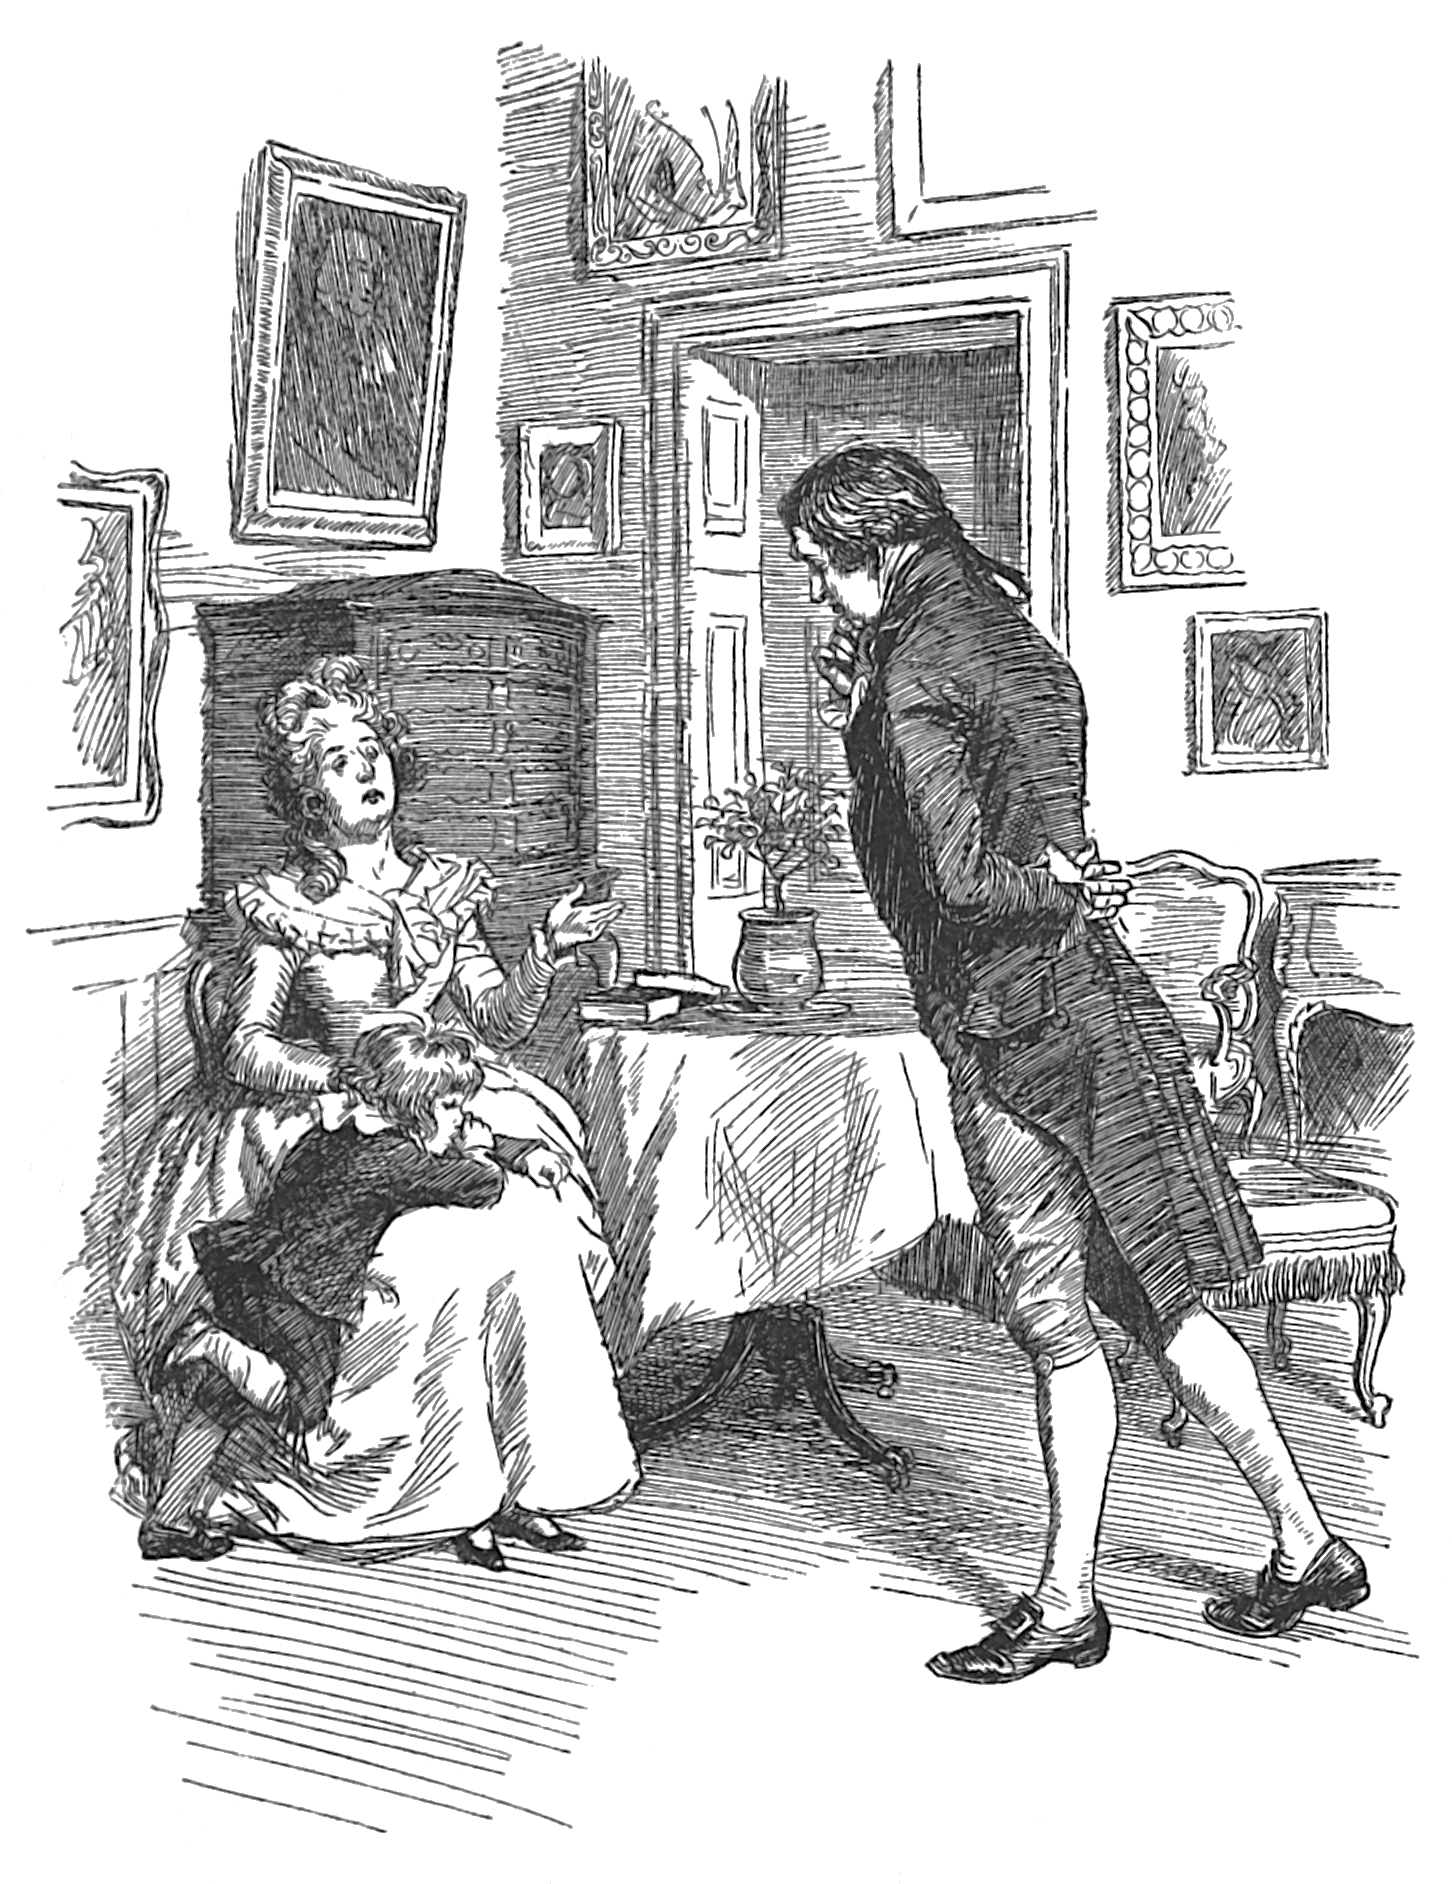
\includegraphics[width=\linewidth]{2half}
% \caption{<I cannot imagine how they will spend half of it>}
% \end{figure}

\begin{bwbigpic}
	[1.0]
	{2half} 
	{<I cannot imagine how they will spend half of it>} 
\end{bwbigpic}

<To be sure it will. Indeed, to say the truth, I am convinced within myself that your father had no idea of your giving them any money at all. The assistance he thought of, I dare say, was only such as might be reasonably expected of you; for instance, such as looking out for a comfortable small house for them, helping them to move their things, and sending them presents of fish and game, and so forth, whenever they are in season. I'll lay my life that he meant nothing farther; indeed, it would be very strange and unreasonable if he did. Do but consider, my dear Mr Dashwood, how excessively comfortable your mother-in-law and her daughters may live on the interest of seven thousand pounds, besides the thousand pounds belonging to each of the girls, which brings them in fifty pounds a year a-piece, and, of course, they will pay their mother for their board out of it. Altogether, they will have five hundred a-year amongst them, and what on earth can four women want for more than that?—They will live so cheap! Their housekeeping will be nothing at all. They will have no carriage, no horses, and hardly any servants; they will keep no company, and can have no expenses of any kind! Only conceive how comfortable they will be! Five hundred a year! I am sure I cannot imagine how they will spend half of it; and as to your giving them more, it is quite absurd to think of it. They will be much more able to give \textit{you} something.>



<Upon my word,> said Mr Dashwood, <I believe you are perfectly right. My father certainly could mean nothing more by his request to me than what you say. I clearly understand it now, and I will strictly fulfil my engagement by such acts of assistance and kindness to them as you have described. When my mother removes into another house my services shall be readily given to accommodate her as far as I can. Some little present of furniture too may be acceptable then.>

<Certainly,> returned Mrs John Dashwood. <But, however, \textit{one} thing must be considered. When your father and mother moved to Norland, though the furniture of Stanhill was sold, all the china, plate, and linen was saved, and is now left to your mother. Her house will therefore be almost completely fitted up as soon as she takes it.>

<That is a material consideration undoubtedly. A valuable legacy indeed! And yet some of the plate would have been a very pleasant addition to our own stock here.>

<Yes; and the set of breakfast china is twice as handsome as what belongs to this house. A great deal too handsome, in my opinion, for any place \textit{they} can ever afford to live in. But, however, so it is. Your father thought only of \textit{them}. And I must say this: that you owe no particular gratitude to him, nor attention to his wishes; for we very well know that if he could, he would have left almost everything in the world to \textit{them}.>

This argument was irresistible. It gave to his intentions whatever of decision was wanting before; and he finally resolved, that it would be absolutely unnecessary, if not highly indecorous, to do more for the widow and children of his father, than such kind of neighbourly acts as his own wife pointed out.